\maketitle
\tableofcontents
\newpage

\begin{otherlanguage}{russian}
  \begin{abstract}
    Пусть есть прибор, который в дискретные моменты времени выдаёт сигнал по закону $f(t) = sin \pi t$. Допустим, наблюдатель зарегистрировал пятьотсчётов в моменты времени $t_{i} = \frac{i}{4}, i = 0, 1, 2, 3, 4$. Задачей наблюдателя(который не знает закона выдачи сигнала) является получение приближённого значения функции на отрезке $[0, 1]$ в любой момент времени.
  \end{abstract}
\end{otherlanguage}

\section{(3) Первое задание}

Используя линейную интерполяцию, найдите значения функции в точках: $t = 0, \frac{1}{6}, \frac{1}{3}, \frac{1}{2}$ и сравните с реальным значением синуса в этих точках. Постройте графики синуса и ломаной, проходящей через пять заданных точек. Отметьте, насколько сильно они различаются в разных частяхграфика. Чем это обусловлено?\\[5mm]

Формула линейной интерполяции:
\[
  f(x) = f(x_{i}) + \frac{f(x_{i+1}) - f(x_{i})}{x_{i+1} - x_{i}}(x - x_{i})
\]

\lstinputlisting{code/first_task.m}
\begin{lstlisting}[backgroundcolor=\color{cyan}]
  y =

        0        0
   0.4714   0.5000
   0.8047   0.8660
   1.0000   1.0000
 \end{lstlisting}

\begin{figure}[h]
  \centering
  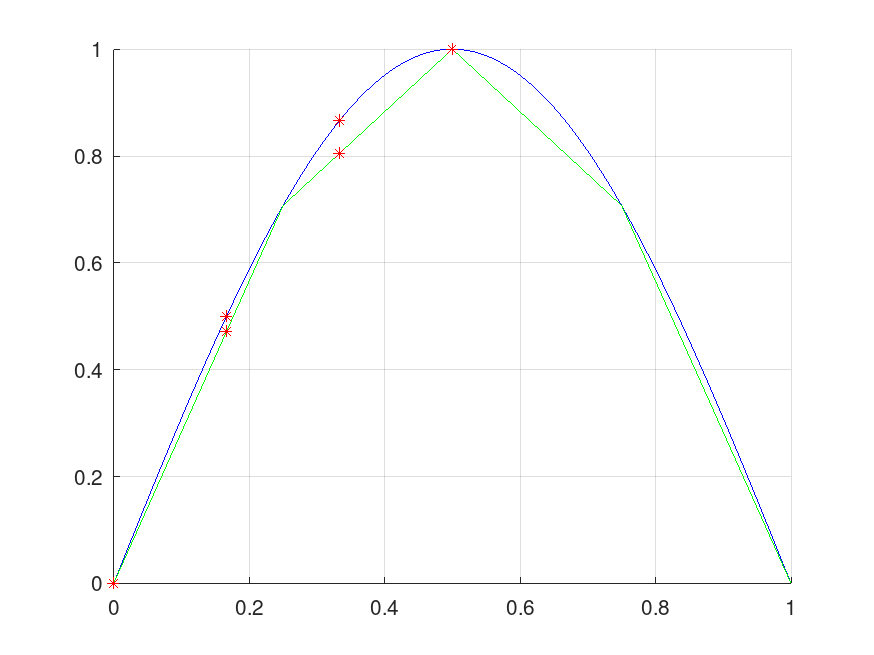
\includegraphics[width=0.8\textwidth]{images/first_task_1.png}
\end{figure}

\section{(3) Второе задание}
Постройте по заданным пяти точкам интерполяционный многочлен Лагранжа или Ньютона и, используя его, найдите значения функции в точках $t =0, \frac{1}{6}, \frac{1}{3}, \frac{1}{2}$. Сравните результаты со значениями, полученными при линейной интерполяции, и значениями синуса в этих точках. Постройте графики синуса и интерполяционного многочлена. Какую максимальную ошибку мы допускаем при аппроксимации синуса данным полиномом? Сравните экспериментальную погрешность с теоретической.\\[2mm]

Воспользуемся формулой:
\[
  L_{n}(x) = \sum_{i=0}^{n}y_{i}\prod_{j=1\\j \neq i}^{n}\frac{x-x_{j}}{x_{i}-x_{j}}
\]
\begin{lstlisting}
f = @(x) sin(pi*x);
i = [0,1,2,3,4];
t1 = i/4;
t2 = [0,1/6,1/3,1/2];
syms x
for i = 1 : length(t1)
	li = 1;
	for j = 1 : length(t1)
		if(j ~= i)
			li = li * (x - t1(j))/(t1(i) - t1(j));
		end
	end
	Li(i) = f(t1(i)) * li;
end

pol = @(x_) eval(subs(sum(Li), x_));

pol(t2)

hold on, grid on;
rx_f = [0 : 0.001 : 1];
rx_p = [0 : 0.1 : 1];
plot(rx_f, f(rx_f), 'k', rx_p, pol(rx_p), 'r')
\end{lstlisting}

Для расчета погрешности:
\[
  R_{n}(x) = f(x)-P_{n}(x) = \frac{y^{(n+1)}}{(n+1)!}\omega_{n+1}(x)
\]
, где $\omega_{n+1}(x) = (x-x_{0})(x-x_{1})(x-x_{n})$
\begin{lstlisting}
A = 1;
for i = 1 : length(t2)
	A = A * (x - t1(i));
end
w = @(x_) subs(A, x_);
df = @(x_) pi*cos(pi*x_);
n = length(t2);
for i = 1 : n;
	err_t(i) = abs(df(t2(i))/factorial(n+1)*w(t2(i)));

	err_e(i) = abs(f(t2(i))) - pol(t2(2));
end
err_t = eval(err_t)
err_e
\end{lstlisting}
\begin{figure}[h]
  \caption{График функции (черным) и полинома (красным)}
  \label{fig:plot_2}
  \centering
  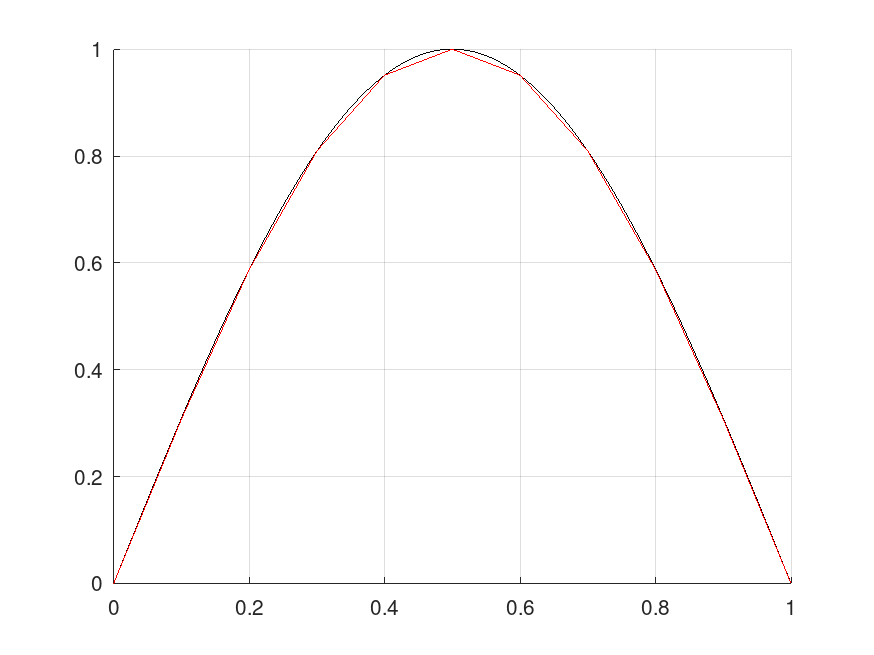
\includegraphics[width=0.8\textwidth]{images/second_task_2.png}
\end{figure}

\section{(4) Третье задание}
В программе сделать возможность строить многочлен Лагранжа или Ньютона для произвольного набора точек $t = t_{0}, t_{1}, \ldots, t_{n}$.\\[2mm]
Уже реализовано

\section{(3) Пятое задание}
Найдите значение интерполяционного полинома при $t = 2$. Почемуоно так сильно отличается от значения синуса в этой точке?\\[2mm]
\begin{lstlisting}
  pol(2)
\end{lstlisting}
\begin{lstlisting}[backgroundcolor=\color{cyan}]
  y =

        0        0
   0.4714   0.5000
   0.8047   0.8660
   1.0000   1.0000
 \end{lstlisting}

\begin{figure}[h]
  \centering
  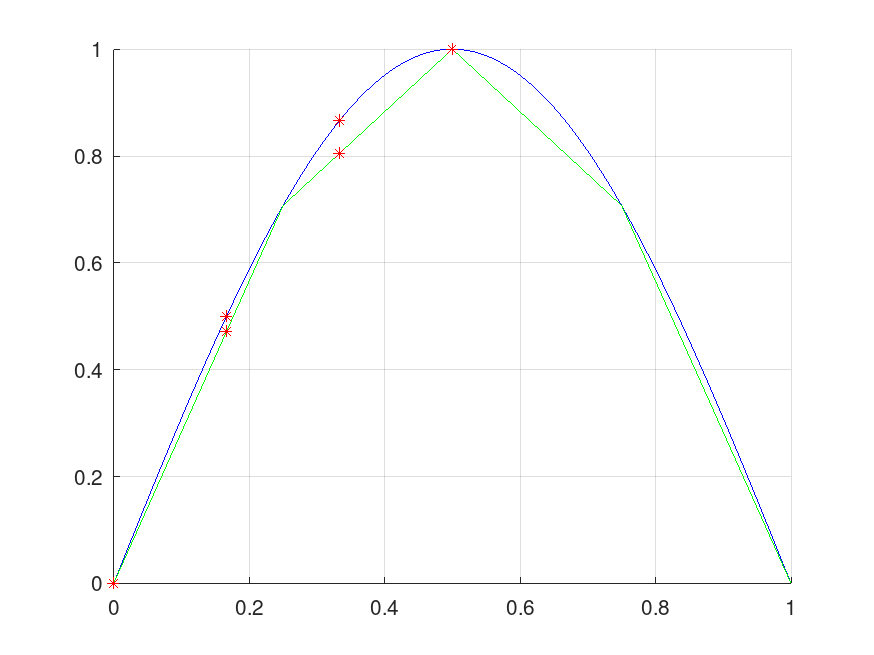
\includegraphics[width=0.8\textwidth]{images/first_task_1.png}
\end{figure}

\section{(3) Второе задание}
Постройте по заданным пяти точкам интерполяционный многочлен Лагранжа или Ньютона и, используя его, найдите значения функции в точках $t =0, \frac{1}{6}, \frac{1}{3}, \frac{1}{2}$. Сравните результаты со значениями, полученными при линейной интерполяции, и значениями синуса в этих точках. Постройте графики синуса и интерполяционного многочлена. Какую максимальную ошибку мы допускаем при аппроксимации синуса данным полиномом? Сравните экспериментальную погрешность с теоретической.\\[2mm]

Воспользуемся формулой:
\[
  L_{n}(x) = \sum_{i=0}^{n}y_{i}\prod_{j=1\\j \neq i}^{n}\frac{x-x_{j}}{x_{i}-x_{j}}
\]
\begin{lstlisting}
f = @(x) sin(pi*x);
i = [0,1,2,3,4];
t1 = i/4;
t2 = [0,1/6,1/3,1/2];
syms x
for i = 1 : length(t1)
	li = 1;
	for j = 1 : length(t1)
		if(j ~= i)
			li = li * (x - t1(j))/(t1(i) - t1(j));
		end
	end
	Li(i) = f(t1(i)) * li;
end

pol = @(x_) eval(subs(sum(Li), x_));

pol(t2)

hold on, grid on;
rx_f = [0 : 0.001 : 1];
rx_p = [0 : 0.1 : 1];
plot(rx_f, f(rx_f), 'k', rx_p, pol(rx_p), 'r')
\end{lstlisting}

Для расчета погрешности:
\[
  R_{n}(x) = f(x)-P_{n}(x) = \frac{y^{(n+1)}}{(n+1)!}\omega_{n+1}(x)
\]
, где $\omega_{n+1}(x) = (x-x_{0})(x-x_{1})(x-x_{n})$
\begin{lstlisting}
A = 1;
for i = 1 : length(t2)
	A = A * (x - t1(i));
end
w = @(x_) subs(A, x_);
df = @(x_) pi*cos(pi*x_);
n = length(t2);
for i = 1 : n;
	err_t(i) = abs(df(t2(i))/factorial(n+1)*w(t2(i)));

	err_e(i) = abs(f(t2(i))) - pol(t2(2));
end
err_t = eval(err_t)
err_e
\end{lstlisting}
\begin{figure}[h]
  \caption{График функции (черным) и полинома (красным)}
  \label{fig:plot_2}
  \centering
  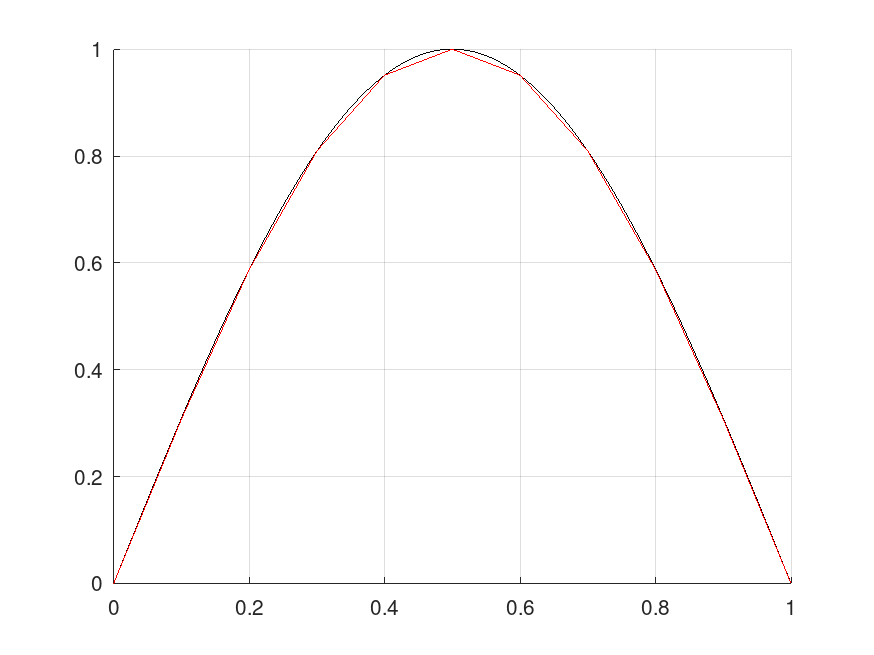
\includegraphics[width=0.8\textwidth]{images/second_task_2.png}
\end{figure}

\section{(4) Третье задание}
В программе сделать возможность строить многочлен Лагранжа или Ньютона для произвольного набора точек $t = t_{0}, t_{1}, \ldots, t_{n}$.\\[2mm]
Уже реализовано

\section{(3) Пятое задание}
Найдите значение интерполяционного полинома при $t = 2$. Почемуоно так сильно отличается от значения синуса в этой точке?\\[2mm]
\begin{lstlisting}
  pol(2)
\end{lstlisting}
\begin{lstlisting}[backgroundcolor=\color{cyan}]
  y =

        0        0
   0.4714   0.5000
   0.8047   0.8660
   1.0000   1.0000
 \end{lstlisting}

\begin{figure}[h]
  \centering
  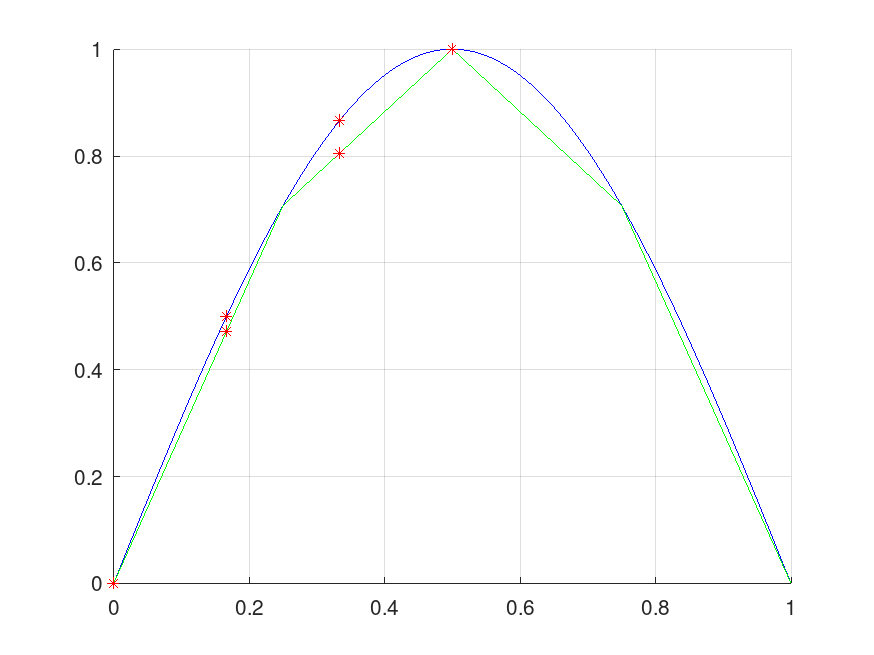
\includegraphics[width=0.8\textwidth]{images/first_task_1.png}
\end{figure}

\section{(3) Второе задание}
Постройте по заданным пяти точкам интерполяционный многочлен Лагранжа или Ньютона и, используя его, найдите значения функции в точках $t =0, \frac{1}{6}, \frac{1}{3}, \frac{1}{2}$. Сравните результаты со значениями, полученными при линейной интерполяции, и значениями синуса в этих точках. Постройте графики синуса и интерполяционного многочлена. Какую максимальную ошибку мы допускаем при аппроксимации синуса данным полиномом? Сравните экспериментальную погрешность с теоретической.\\[2mm]

Воспользуемся формулой:
\[
  L_{n}(x) = \sum_{i=0}^{n}y_{i}\prod_{j=1\\j \neq i}^{n}\frac{x-x_{j}}{x_{i}-x_{j}}
\]
\begin{lstlisting}
f = @(x) sin(pi*x);
i = [0,1,2,3,4];
t1 = i/4;
t2 = [0,1/6,1/3,1/2];
syms x
for i = 1 : length(t1)
	li = 1;
	for j = 1 : length(t1)
		if(j ~= i)
			li = li * (x - t1(j))/(t1(i) - t1(j));
		end
	end
	Li(i) = f(t1(i)) * li;
end

pol = @(x_) eval(subs(sum(Li), x_));

pol(t2)

hold on, grid on;
rx_f = [0 : 0.001 : 1];
rx_p = [0 : 0.1 : 1];
plot(rx_f, f(rx_f), 'k', rx_p, pol(rx_p), 'r')
\end{lstlisting}

Для расчета погрешности:
\[
  R_{n}(x) = f(x)-P_{n}(x) = \frac{y^{(n+1)}}{(n+1)!}\omega_{n+1}(x)
\]
, где $\omega_{n+1}(x) = (x-x_{0})(x-x_{1})(x-x_{n})$
\begin{lstlisting}
A = 1;
for i = 1 : length(t2)
	A = A * (x - t1(i));
end
w = @(x_) subs(A, x_);
df = @(x_) pi*cos(pi*x_);
n = length(t2);
for i = 1 : n;
	err_t(i) = abs(df(t2(i))/factorial(n+1)*w(t2(i)));

	err_e(i) = abs(f(t2(i))) - pol(t2(2));
end
err_t = eval(err_t)
err_e
\end{lstlisting}
\begin{figure}[h]
  \caption{График функции (черным) и полинома (красным)}
  \label{fig:plot_2}
  \centering
  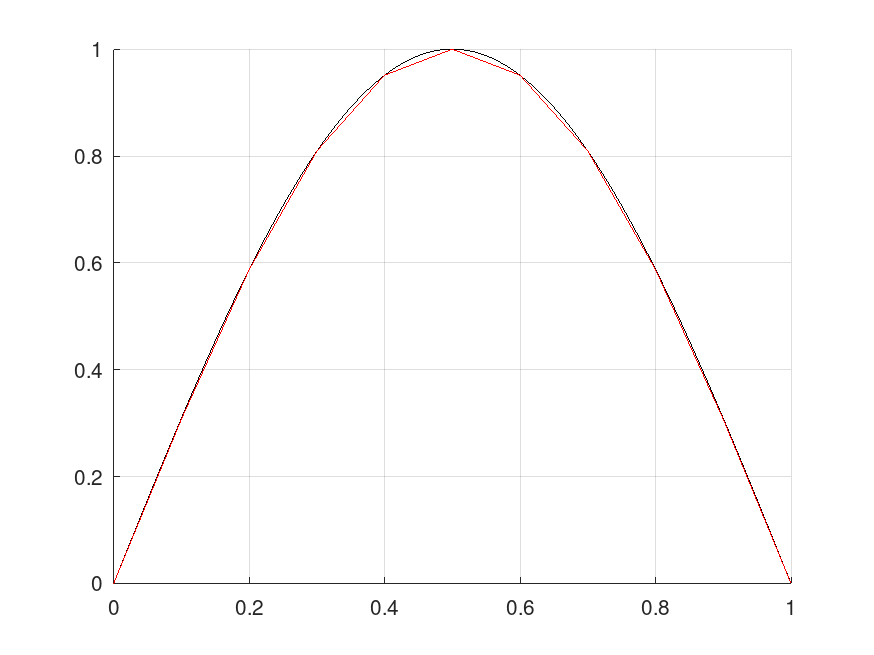
\includegraphics[width=0.8\textwidth]{images/second_task_2.png}
\end{figure}

\section{(4) Третье задание}
В программе сделать возможность строить многочлен Лагранжа или Ньютона для произвольного набора точек $t = t_{0}, t_{1}, \ldots, t_{n}$.\\[2mm]
Уже реализовано

\section{(3) Пятое задание}
Найдите значение интерполяционного полинома при $t = 2$. Почемуоно так сильно отличается от значения синуса в этой точке?\\[2mm]
\begin{lstlisting}
  pol(2)
\end{lstlisting}

\begin{lstlisting}[backgroundcolor=\color{cyan}]
  ans = 8.4710
\end{lstlisting}

\begin{lstlisting}
  f(2)
\end{lstlisting}

\begin{lstlisting}[backgroundcolor=\color{cyan}]
  ans = -2.4493e-16
\end{lstlisting}
